For this project we worked in pair with a partner, my partner was Valentin Lecompte, ens18vle.
We did not fully separate our work in two but my partner focused more on the electronic part of the project while I was more focused on the development part. 

My report will then describe the program where my partner's report will talk about the electronic part and describe also the structure of the robot.

The used hardware for this project is 1 button, 2 leds, 1 potentiometer, 2 DC motors, a level shifter, a numeric to analogy converter, a level converter, a IR sensors array and a Beaglebone.

The developed program uses the PyBBIO library, used as an interface between the code and the hardware.

All the source code can be found here: \href{http://github.com/ThomasRanvier/line_following_robot}{link to my github}.

\section*{Linking the motors to the Beaglebone}

The first task that we had to do was to be able to control the motors as we want.
The introductory lab helped us a lot since we now knew that we had to develop a PI controller to control the motor more easily.

We connected the motors to the Beaglebone, we use two PWM pins to send the power that will make their speed vary and we get the results from their encoders through the 2 specialised pairs of EQEP pins.

\subsection*{Encoders}

I initially tried to implement the encoder entirely by myself.
The main issue was that I used normal pins on the Beaglebone because I did not know that we had to use specialised pins for this.
The result was that the encoder that I implemented worked most of the time but sometimes the pins were not able to receive the informations from the motors quick enough and so the result was not constantly good.

After that, to implement the encoders I used the RotaryEncoder object from the PyBBIO library.
With this object we can easily recuperate the position of the encoder.

I created a class named Encoder to use more simply the RotaryEncoder object.
I also scale the result of the RotaryEncoder between 0 and 255 by multiplying it by a gain defined as $\dfrac{255}{8000}$.

\subsection*{PI controllers}

To implement the PI controllers I created a PI\_controller class, it is used to instantiate a PI controller with the $P$ and $K$ values that we want.
The role of the PI controller is to take the encoder output as entry and return the speed to send to the linked motor in order to get the closest possible to a defined speed.

The speed that we want to achieve is called the $wanted\_speed$ and it can be set through the $set\_wanted\_speed$ function.

We can also set the limits of the PI controller, we used $0$ and $255$ as limits since the values that we can send through the PWM pins are on one Byte.

We used the step measurement that we did on the first lab to set the $P$ and $I$ values of the PI controller:

\begin{align*}
    &P \simeq 1.00726
    &I \simeq 18.38404
\end{align*}

\section*{Read and analyse the Infra-Red sensors values}

Once we were able to control both the motors as desired we had to read and analyse the informations from the IR sensors to automatically set the wanted speeds of the two PI controllers to make the robot follow the line.

\subsection*{Recuperate the informations}

The IR sensors informations can be recuperated from the SPI pins, it uses an analogy to numerical hardware converter.

In order to get the informations from the IR sensors and put them into a nice usable form I created the IR\_sensors class, it is used as an interface between the program and the IR sensor array.

This class contains a 'private' method called '\_\_adc\_read', it returns the raw informations from the 8 IR sensors, it is used in the public 'get\_activations' method which can be used by the user.

This last function returns the informations in a dictionary which contains the current and also the last activation.
The current activation is a list of 8 digital values, I used an arbitrary threshold value of 300 and all the raw values from the '\_\_adc\_values' that are above the threshold are converted to 1 and all the ones under are converted to 0.
It makes it very easy to know what sensor is activated or not.

The last activation is of the same form, a list of 8 digital values, but instead of the current activation it is the last activation, meaning the last time that we detected an activated sensor.
Indeed this list is used when the current activation detects nothing, it means that the robot is out of the line, when in that case we need to know in what direction it exited the line so that we can make it turn in the right direction.

\subsection*{Analyse the informations}

Once we get the current and last activation in a nice form we need to analyse them.

This analyse takes place in the robot class, it uses some pre-defined values:

\begin{align*}
    &ir\_sensor\_weights = [-9, -7, -5, -1, 1, 5, 7, 9]\\
    &ir\_sensor\_max\_weight = 12\\
\end{align*}

We have three cases.

\subsubsection*{First case}

The 8 values of the current IR activation are at 1.
It basically means that all the IR sensors are detecting no surface under them.
It means that the robot is lifted up the ground, to move it elsewhere for example.
In that case we set the wanted speed of both the PI controllers to 0, it makes the robot stop moving.

\subsubsection*{Second case}

The 8 values of the current IR activation are at 0.
It means that the robot detects ground but no line, it is when the last activation will be useful.
We have to use the last activation to figure out in what direction to turn so we can get back to the line.
There are three cases:
\begin{enumerate}
    \item The most extreme sensor on the right was previously activated, it means that the robot exited the line by going to the left, we have to make it turn on the right.
        To do so we slow down the right wheel by using this formula $ir\_sensor\_max\_weight \cdot scale \cdot speed$.
        Here the $speed$ value is the speed that we ideally want the robot to always go and the $scale$ is a defined value that will make the opposite wheel slow more or less depending on its value.
        The value that we usually use for the $scale$ is $\dfrac{1}{ir\_sensor\_max\_weight}$, it makes the opposite wheel stop totally in the case where the robot is out of the line.
    \item The most extreme sensor on the left was previously activated, it means that the robot exited the line by going to the right, we have to make it turn on the left.
    \item The last case is when none of the above were activated, it means that the line stopped under the robot, then the robot should continue straight forward to reach the line when it starts again further away.
\end{enumerate}

\subsubsection*{Last case}

Else we have to analyse the current IR activation more precisely.
The first thing is to compute the weight of the current activation, the used function takes into entry the current activation.
The activation list is divided in two, it only takes into account the most extreme activation on the right and on the left.
This is the pseudocode of the function so it is easier to understand how it works:

\FloatBarrier
\begin{algorithm}
    \caption{Compute the weight given an IR activation}
    \label{compute_ir_weight}
    \begin{algorithmic}[1]
        \Procedure{$\_\_compute\_ir\_weight$}{$activation$}
            \State $weight \gets 0$
            \For{$i\texttt{ }in\texttt{ }range(0, 4)$}
                \If{$activation[i] == 1$}
                    \State $weight \gets weight + ir\_sensor\_weights[i]$
                    \State \textbf{break}
                \EndIf
            \EndFor
            \For{$i\texttt{ }in\texttt{ }range(7, 3, -1)$}
                \If{$activation[i] == 1$}
                    \State $weight \gets weight + ir\_sensor\_weights[i]$
                    \State \textbf{break}
                \EndIf
            \EndFor
            \State \textbf{return} $weight$
        \EndProcedure
    \end{algorithmic}
\end{algorithm}
\FloatBarrier

With this computed weight we know that if it is positive we have to make the robot turn to the right and conversely.
The speed of the opposite wheel is then computed in that way: $speed - (scale \cdot abs(weight) \cdot speed)$.

\section*{Results and improvements}

Our robot is able to follow the line, go straight forward if the line suddenly stops and go in the right direction if it goes out of the line in a sharp turn.
Under is a picture of the robot.

\begin{figure}[h]
    \centering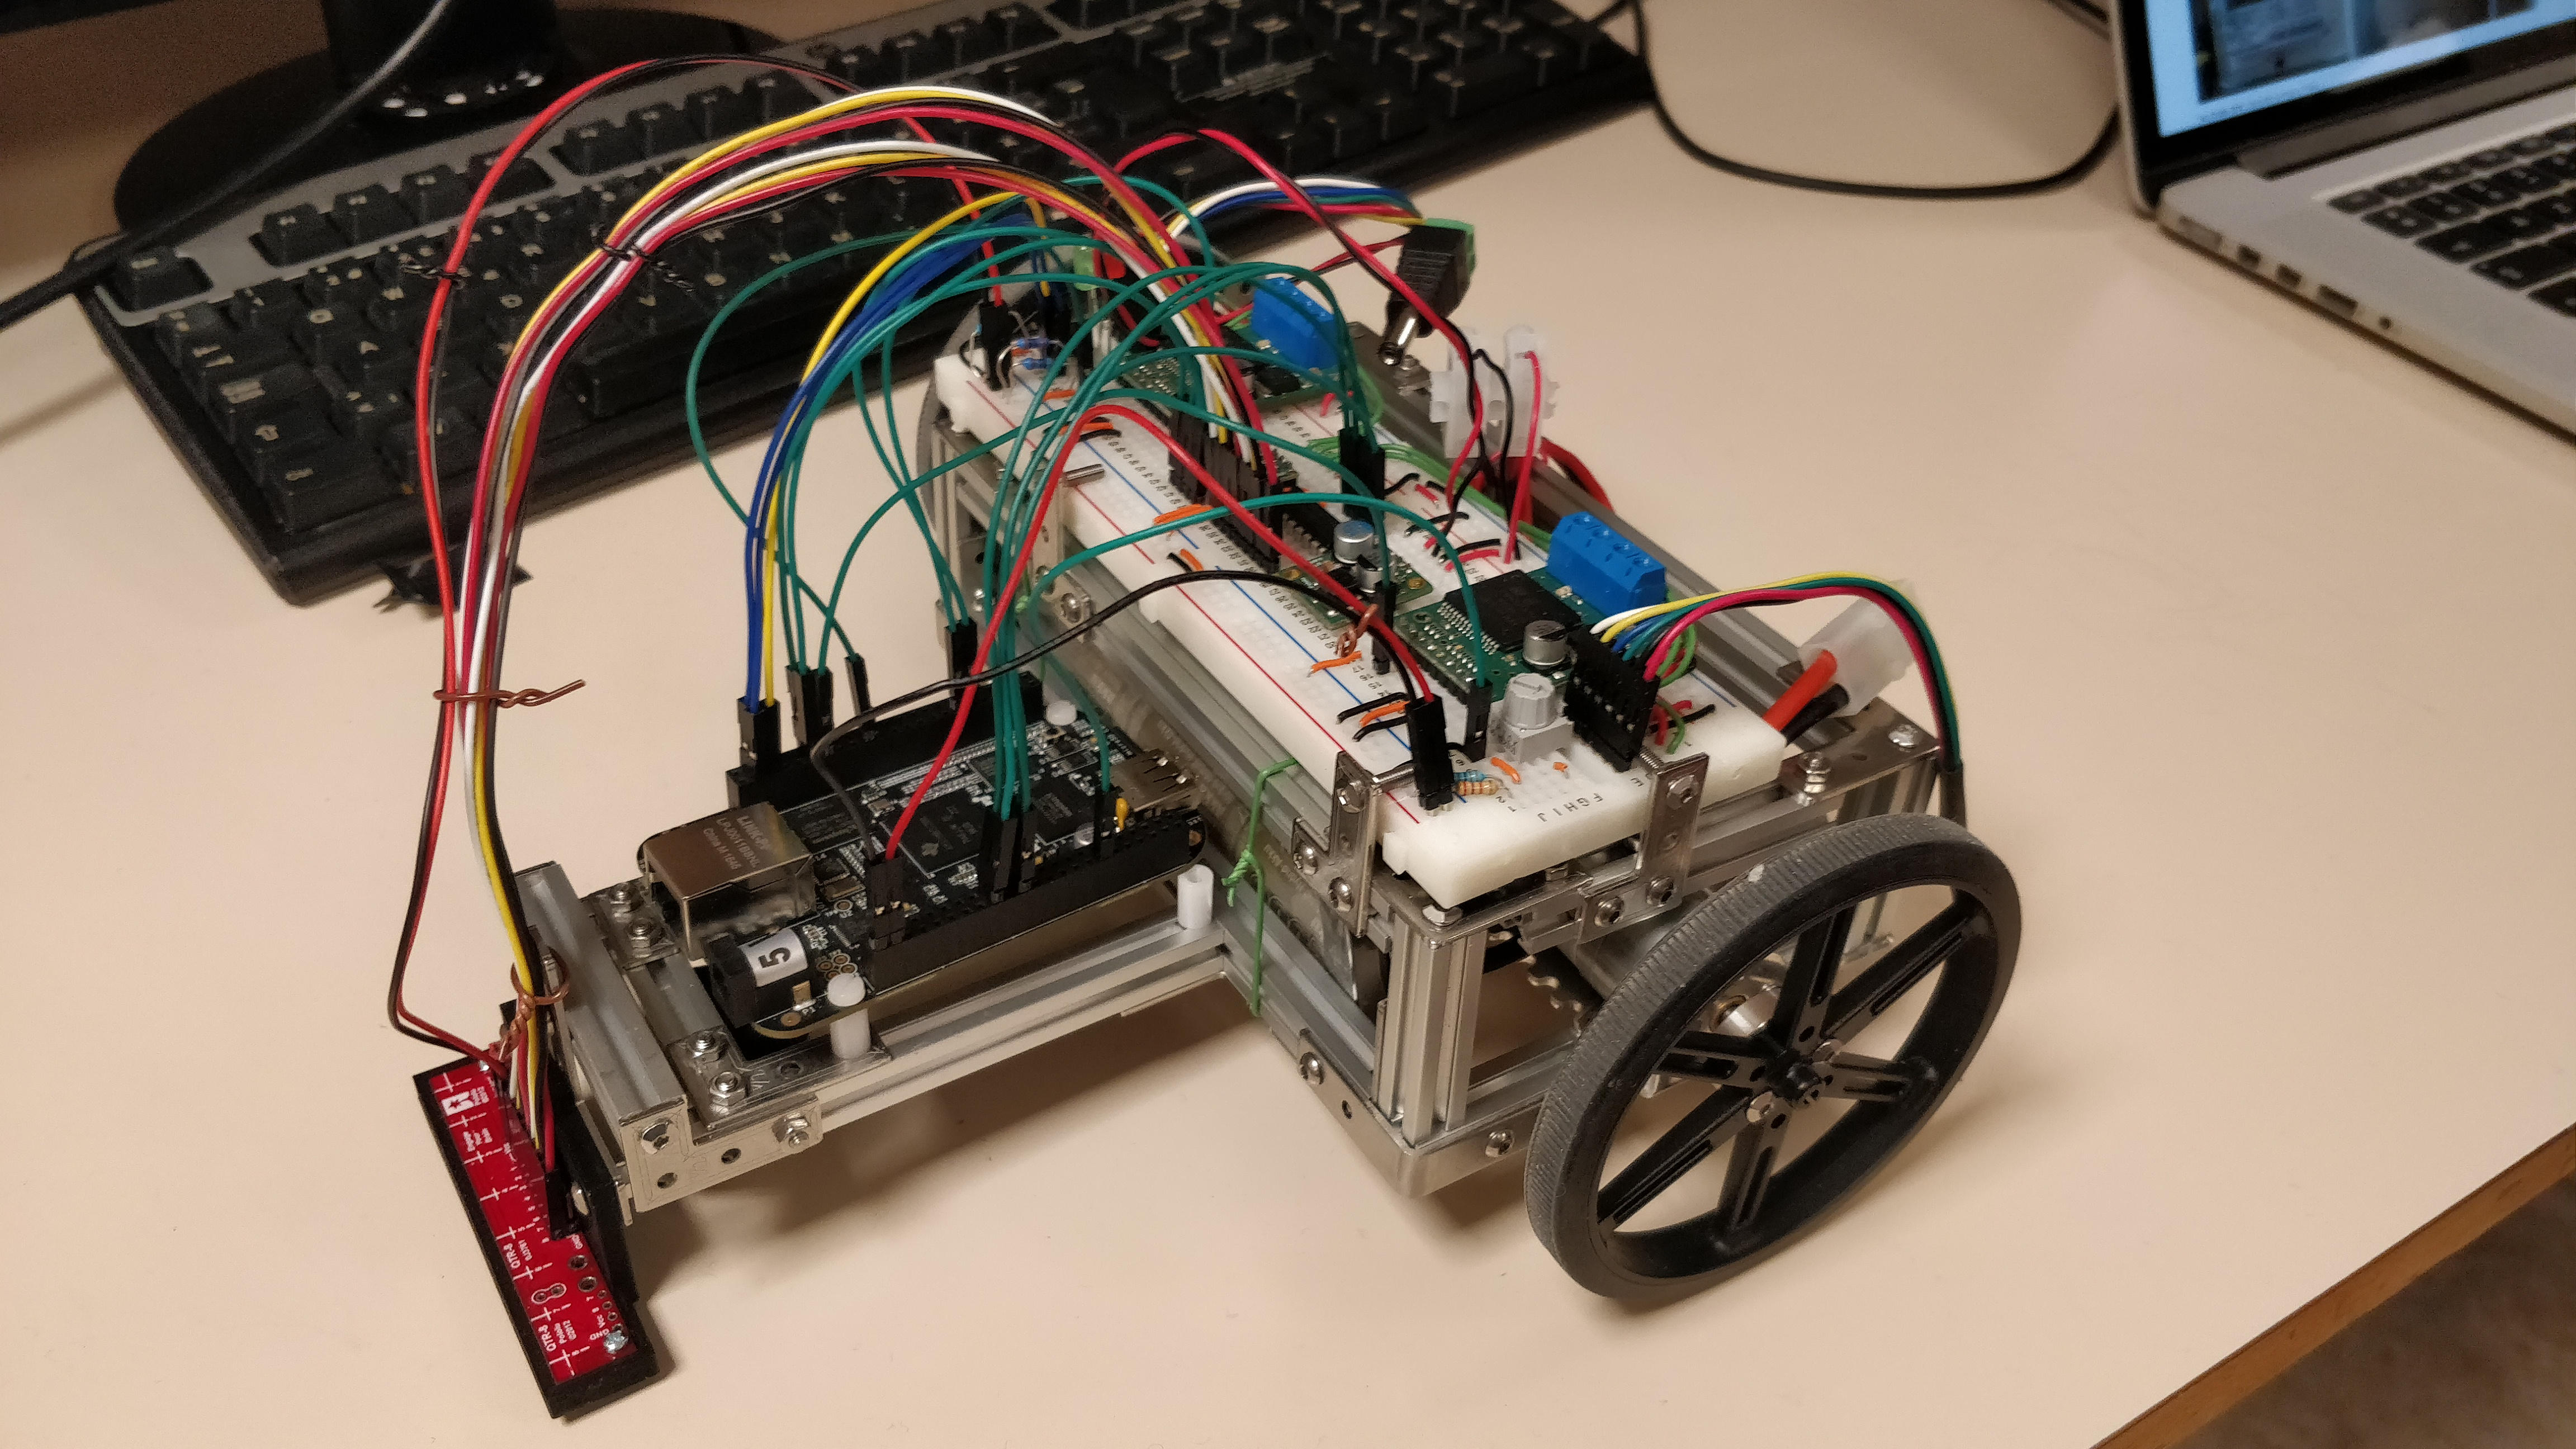
\includegraphics[width=0.5\textwidth]{robot.jpg}
\end{figure}

\subsection*{The lines in parallel}

In one of the two circuits there is a part of the road where there are three lines in parallel, if the robot is not exactly on the right line it will eventually detect one of the two others.
In that case since we only consider the extreme values of our sensors the robot would sometimes suddenly turn into an other direction.
To fix this issue I added a function that detects when there are more than one line detected.
In that case the negative weights become positive and conversely, this will make the robot turn in the other way.
The result is that it will avoid going on the parasite lines.

\subsection*{Various improvements}

We added some functionalities that make it easier to use the robot when it is not connected to a computer.
We added one green LED, one red LED, one button and one potentiometer.

When the Beaglebone starts our programs is started as a daemon, when the program starts the two LEDs blink simultaneously until the button is pressed.

Once the button has been pressed the main function is launched, it will create all the instances to control the robot and when everything is ready the green LED goes on, at that point the robot is in pause so nothing else will happen.

When the green LED is on we can press once again the button, it will light on the red LED to signal the state of the robot and it will make the robot start reading the IR sensors datas and start following the line if there is one to follow.
When we want to stop the robot we can press the button again, the red LED goes off.

We also added a potentiometer, it makes the speed of the robot vary between 0 and 255.

\subsection*{Possible improvements}

There are a lot of possible improvements to do, we could have added ultra-sonic sensors to try and detect obstacles.
We could also have added a screen to make it easier to use the robot by displaying interesting informations.
